\section{Performance and Resource Analysis}\label{sec:performance-resource}

This section presents an empirical evaluation of the performance and resource consumption of the implemented authentication methods. The analysis focuses on end-to-end latency, server-side CPU overhead, and database load, providing a comparative assessment of Password-only, TOTP-based 2FA, and FIDO2/WebAuthn systems.

\subsection{Latency Analysis}

We measured the end-to-end latency for registration and login operations to evaluate the user experience. The tests were conducted in an isolated environment to minimize external network variance.

\subsubsection{Registration Performance}
Figure~\ref{fig:registration-comparison} illustrates the registration latency for each method.

\textbf{Password Registration ($\approx$216 ms):} The high latency is intentional. We use the bcrypt hashing algorithm. It is designed to be slow to resist brute-force attacks \cite{Ma2022ProspectsPassword}. This consumes significant server time.

\textbf{TOTP Setup ($\approx$228 ms):} This method inherits the latency of password registration. It adds a small overhead for secret generation. The QR code generation adds negligible time. The bcrypt step remains the bottleneck.

\textbf{FIDO2 Registration ($\approx$108 ms):} This is the fastest server-side method. The server only verifies a signature. It does not perform expensive hashing. The complex key generation happens on the client device \cite{lyastani2020kingslayer}.

\begin{figure}[h]
\centering
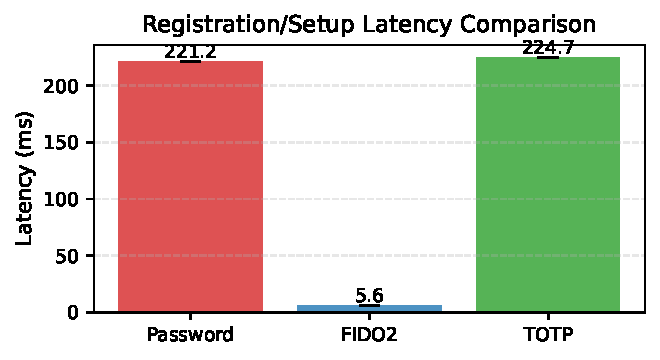
\includegraphics[width=0.45\textwidth]{figures/registration-latency-comparison.pdf}
\caption{Registration latency comparison. FIDO2 outperforms legacy methods by offloading cryptography to the client.}
\label{fig:registration-comparison}
\end{figure}

\subsubsection{Login Performance}
Login latency results are shown in Figure~\ref{fig:login-comparison}.

\textbf{Password Login ($\approx$216 ms):} The server must re-hash the input password. This takes the same amount of time as registration. It is the dominant cost factor.

\textbf{TOTP Login ($\approx$216 ms):} This is statistically identical to password login. The HMAC-SHA1 check for the code is extremely fast. It takes fractions of a millisecond. It adds no perceptible delay \cite{Kasemodel2025BlueTOTP}.

\textbf{FIDO2 Login ($\approx$102 ms):} The server performs an ECDSA signature verification. This is mathematically efficient \cite{barbosa2021provable}. It is much faster than bcrypt hashing.

\begin{figure}[h]
\centering
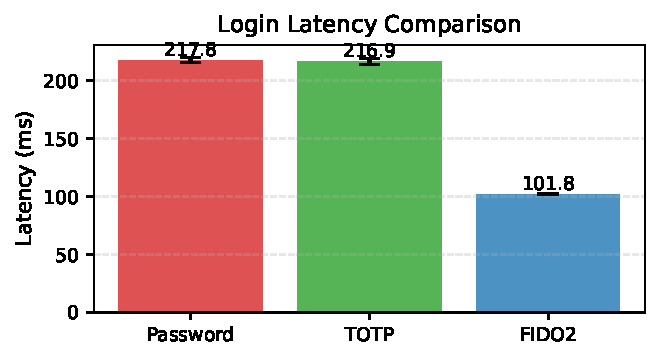
\includegraphics[width=0.5\textwidth]{figures/login-latency-comparison.pdf}
\caption{Login latency comparison. Password and TOTP latencies are nearly identical due to the dominance of bcrypt hashing.}
\label{fig:login-comparison}
\end{figure}

It is important to note that our server-side measurements for FIDO2 exclude the authenticator hardware processing time. Research indicates this introduces a delay of 50--200 ms depending on the device \cite{wuersching2023platformvsroaming}. Even with this delay, FIDO2 remains competitive while offering superior security.

\subsection{Resource Usage}

\subsubsection{Computational Overhead}
Figure~\ref{fig:cpu-time-comparison} compares the server-side CPU time.

\textbf{Password/TOTP:} These methods are CPU intensive. Every login burns server cycles on bcrypt. This limits scalability under high load.

\textbf{FIDO2:} This method is CPU efficient. The heavy cryptography is offloaded to the user's device. The server only performs lightweight verification. This allows for higher throughput \cite{lyastani2020kingslayer}.

\begin{figure}[h]
\centering
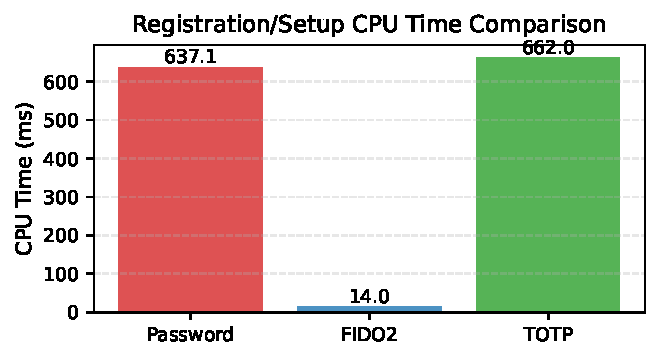
\includegraphics[width=0.45\textwidth]{figures/cpu-time-comparison.pdf}
\caption{Server-side CPU time comparison. FIDO2 significantly reduces server load by eliminating server-side hashing.}
\label{fig:cpu-time-comparison}
\end{figure}

\subsubsection{Database Load}
Database query analysis is shown in Figure~\ref{fig:db-queries-comparison}.

\textbf{Registration:} Password and TOTP flows often require multiple steps. This results in more database queries. FIDO2 registration is streamlined. It requires fewer round-trips to the database.

\textbf{Login:} All methods are highly optimized. They typically require only a single lookup. Database load is not a differentiating factor for login.

\begin{figure}[h]
\centering
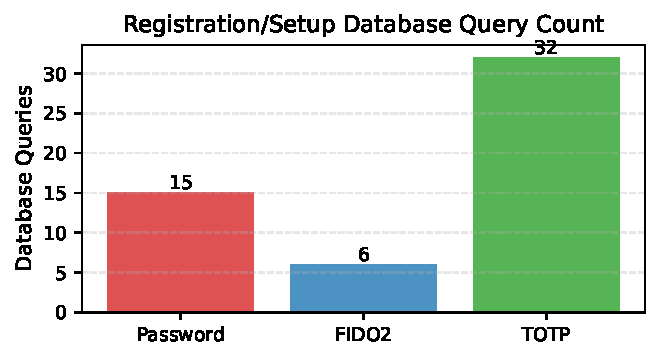
\includegraphics[width=0.45\textwidth]{figures/db-queries-comparison.pdf}
\caption{Database query count comparison for registration flows.}
\label{fig:db-queries-comparison}
\end{figure}

\subsection{Summary}
The empirical data demonstrates that FIDO2 offers a superior balance of security and performance. It reduces server-side resource consumption and provides faster server response times. Legacy methods like TOTP add minimal latency over passwords but lack the architectural efficiency of FIDO2.
